\begin{figure}[!ht]
    \centering
    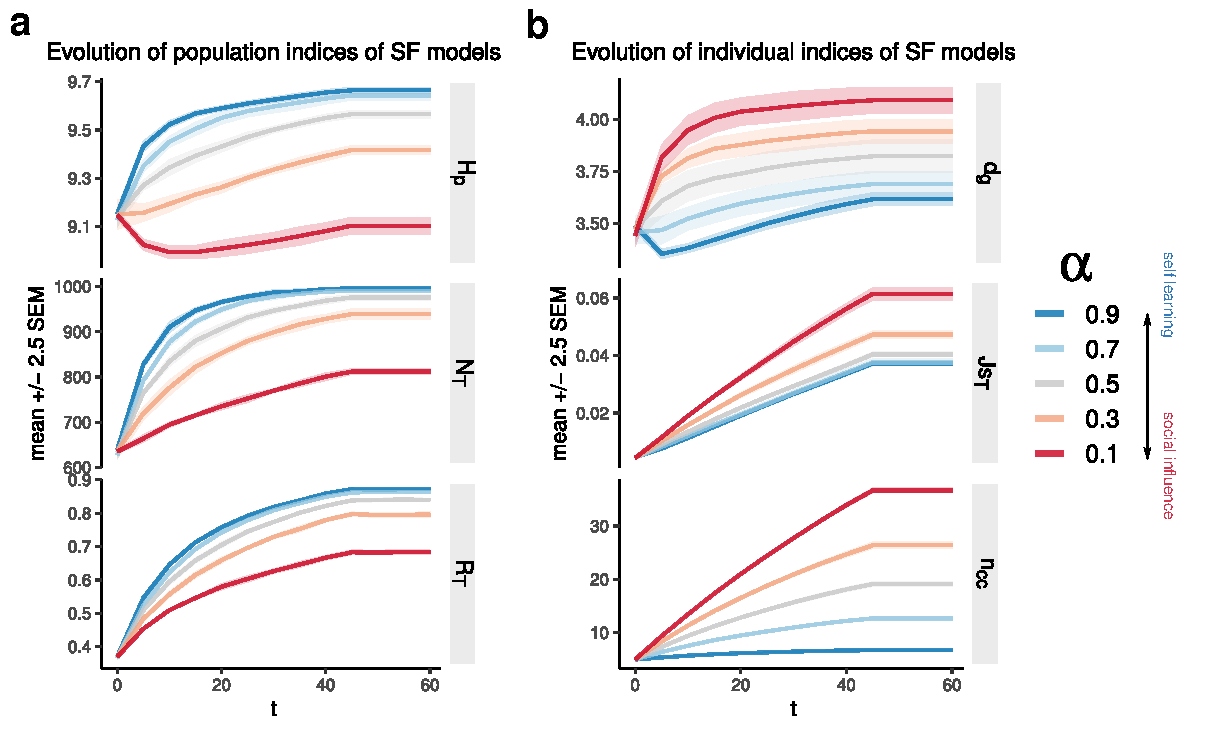
\includegraphics[width=\textwidth]{figures/Fig2.pdf}
    \caption{
    \textit{Changes of population topic diversity indices} (\textbf{a}) \textit{and of individual diversity indices} (\textbf{b}) \textit{of the scale-free (SF) intralayer models} \textit{due to} $\alpha$. $H_p$: topic population entropy; $N_T$: number of distinct topics; $R_T$: robustness due to \textit{random} removal of agents; $d_g$: mean distance of the subset of topics that agents know; $Js_T$: Jaccard similarity of topic set between agents; $n_{cc}$: number of connected components of induced subgraphs based on each agent's learnt topics. See \textbf{Sect. \ref{sec:method-diversity}} and \textbf{Fig. \ref{fig:1}}d,e for more details. Each line represents the mean changes of 5 realizations, analyzed every 5 steps.
    }
    \label{fig:2}
\end{figure}